\glsreset{WCA}
\gls{WCA} refers to a novel category of wearable and mobile immersive applications which aim to amplify human cognition in both day-to-day tasks and professional settings.
\glspl{WCA} work in a mode analogous to how \gls{GPS} navigation systems guide drivers, by seamlessly providing relevant instructions and feedback relating to the current task at hand and staying out of the way of the user when guidance is not required.
These applications operate much like a human assistant would, by observing the performance of the user and offering guidance proactively.
Through the use of sensors (most commonly video inputs), the application follows the progress of the task in realtime by continuously sampling the state of the physical system.
The input is parsed to an internal symbolic representation of the state of the task;
whenever a change of state is detected the application provides appropriate feedback or instructions to the user.
This feedback can be in the form of text, images, video, and/or audio, and guides the user towards the next desired system state.
If no change in state is detected, the application remains silent and out-of-the-way.
In other words, the application silently discards samples which capture an intermediate or unfinished state, or simply are too noisy to be processed.
\Cref{fig:wca} illustrates this mode of operation in a \gls{WCA} guiding a user to manipulate a structure composed of LEGO bricks.

\begin{figure}
    \centering
    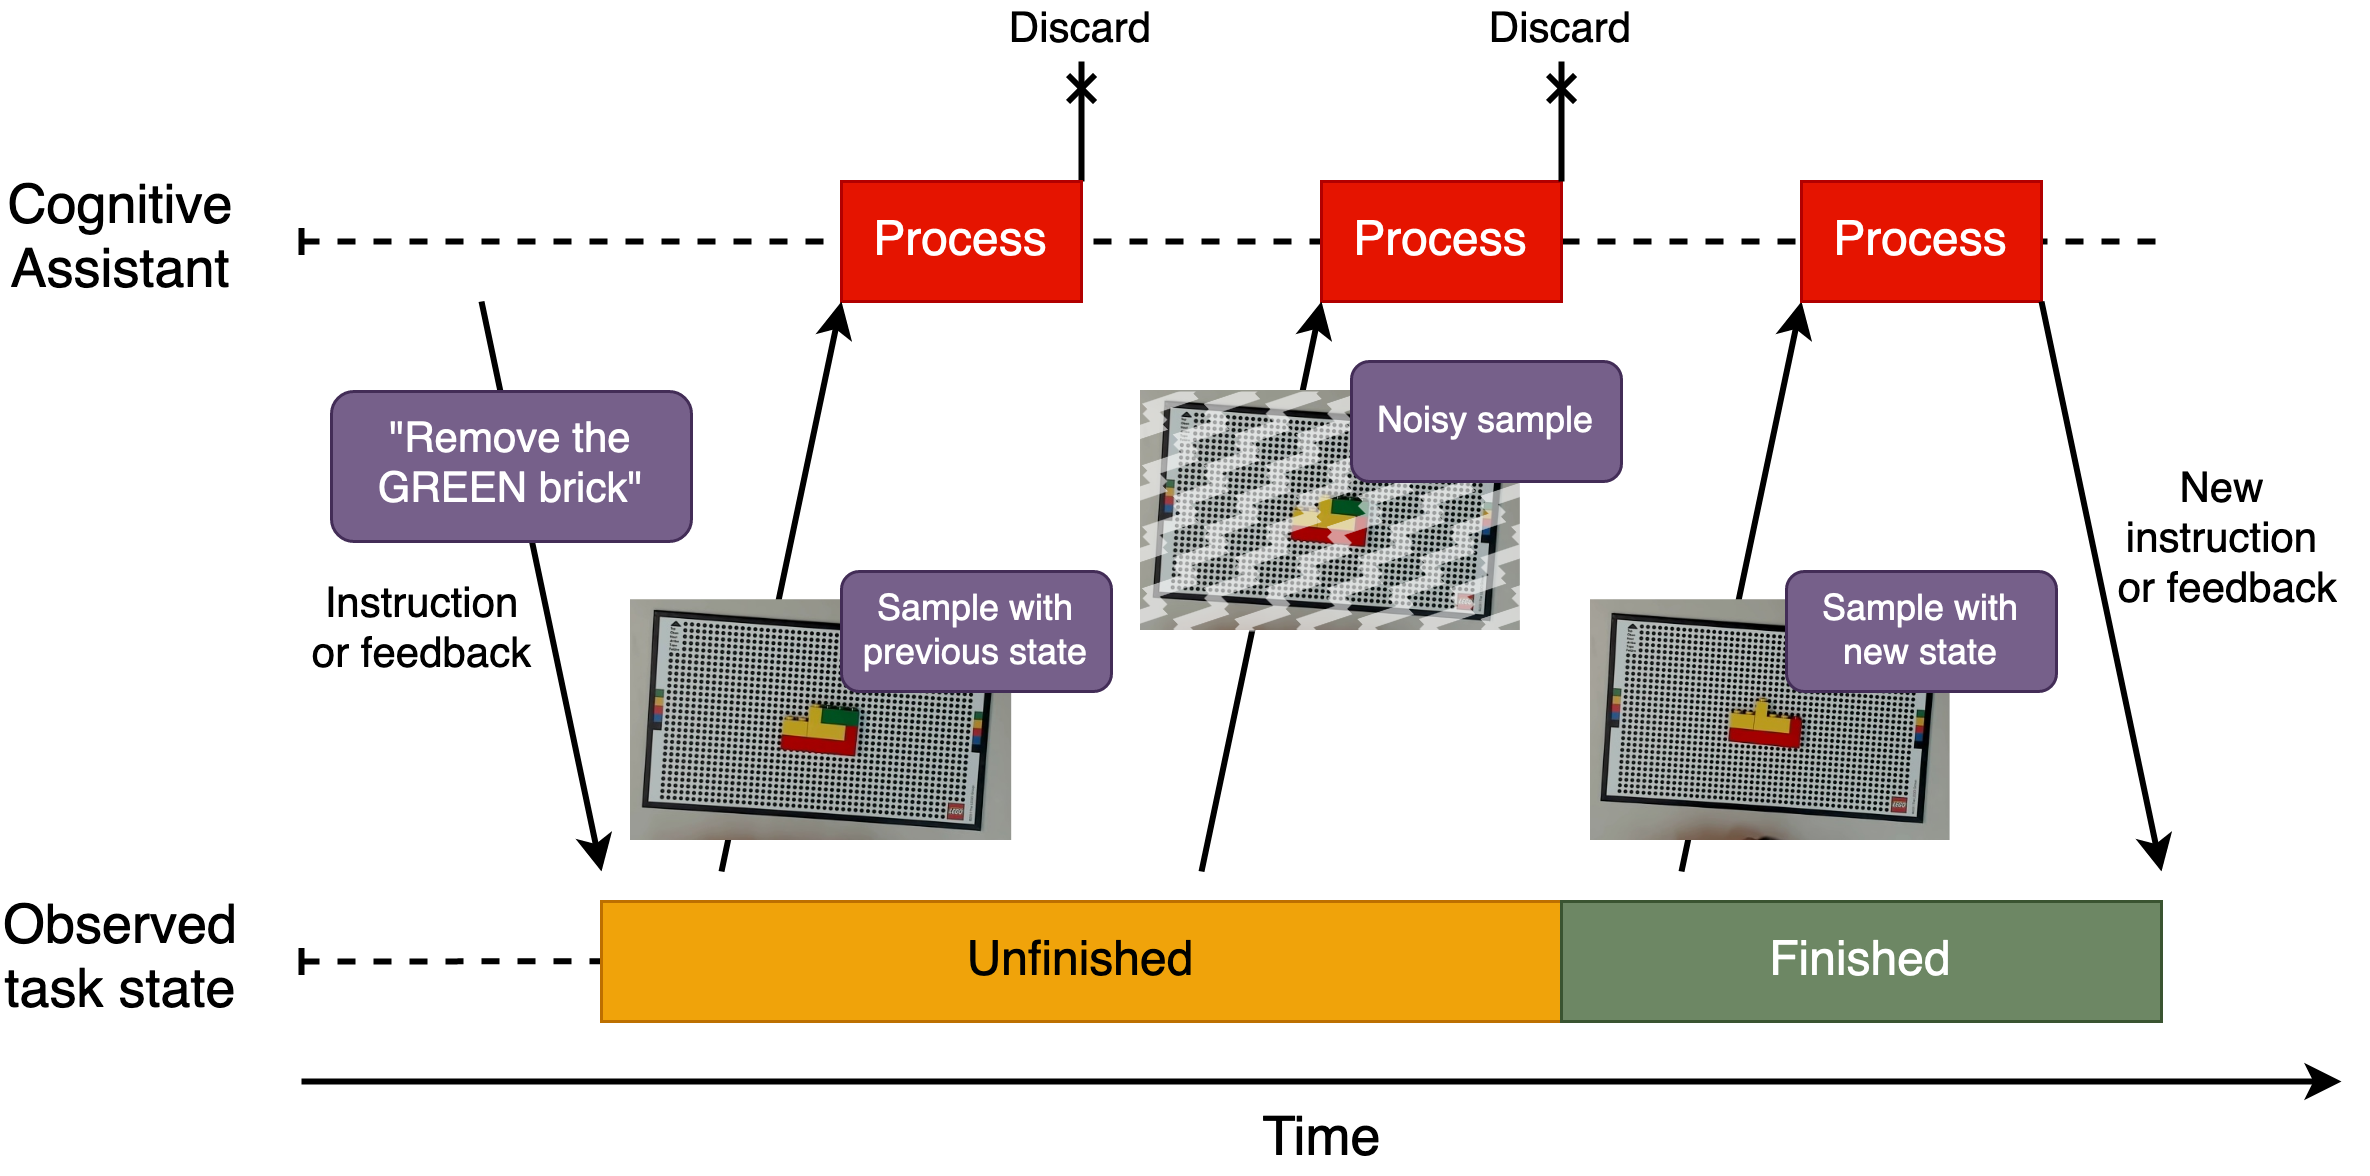
\includegraphics[width=.9\textwidth]{Figs/wca_state}
    \caption{%
        Mode of operation of \acs{WCA} applications.
        The assistant continuously samples the state of the monitored task, and provides appropriate feedback once a state change has been detected.
        Samples that do not result in feedback are silently discarded.
    }\label{fig:wca}
\end{figure}

As the name implies, \glspl{WCA} are available whenever the user requires them, without being tethered to a particular physical location;
they are pervasive and mobile~\cite{ha2014towards}.
This leads to interesting consequences for \gls{WCA} system design when combined with their requirement of seamless integration with the context of the user.
The wearable nature of \gls{WCA} directly implies use of lightweight and battery-powered devices, greatly constrained in terms of energy and computing resources.
The requirements of immersive and seamless interaction, on the other hand, suggest a level of context sensitivity and proactivity that can only be provided by real-time analysis of sensor inputs such as video and audio feeds.
This kind of compute- and energy-intensive processing, often involving \gls{ML} algorithms and \glspl{DNN}, is unfeasible to be performed on wearable devices, and thus these applications \emph{must} necessarily make use of compute offloading~\cite{ha2014towards,wang2020scaling}.

However, it is understood today the cloud represents an unsuitable candidate for offloading computation in these applications, given the high latencies involved.
Given their immersive nature, feedback in \gls{WCA} systems should be provided ``quickly'' (relative to the task at hand), as users will have expectations of constant and immediate feedback as they interact with the system.
As is the case for most \gls{XR} applications, delayed feedback in \gls{WCA} can have severe negative consequences for the quality of the user experience.
Depending on the task, these consequences can range from simply distracting or annoying the user (in the case of less interactive tasks such as step-by-step assembly), to actively handicapping user performance (in the case of highly interactive tasks).
There is therefore a broad understanding today that edge computing is a key enabling technology for \gls{WCA} applications~\cite{ha2014towards,wang2020scaling,chen2018application,olguinmunoz2021impact}.

\medskip
In literature, research on \gls{WCA} has focused mostly on the implementation of prototype applications and platforms.
\citeauthor{ha2014towards}~\cite{ha2014towards} coined the term \acl{WCA} in\ \citeyear{ha2014towards}.
Their work described a first prototype system employing a Google Glass wearable device, and identified the challenges of offloading the computation for such an application to the cloud.
The authors were originally inspired by assistive use cases for people suffering from some form of cognitive decline due to aging, illness, or traumatic brain injury~\cite{ha2014towards,satyanarayanan2019augmenting}.
More recently, the scope of \glspl{WCA} has been expanded to include a broader range of use cases, including complex assembly tasks~\cite{chen2017empirical,chen2018application,wang2020scaling,wang2019towards}.
\cite{chen2015early} and~\cite{chen2018application} further developed the platform described in~\cite{ha2014towards}, and produced a number of different assistive applications such as the aforementioned LEGO assistant, and others such as a Ping-Pong assistant capable of providing real-time hints to players of table tennis, and more advanced assembly assistant for IKEA furniture.
Yet another platform for \gls{WCA} was introduced in~\cite{chatzopoulos2017hyperion}, with the goal of providing real-time contextual information in text-form to users.
Furthermore, important work has been done in the implementation of such systems for industrial and factory applications~\cite{belletier2021wearable}.
Non-wearable cognitive assistance systems for assembly tasks have already been proven to be valuable tools in the industrial workplace~\cite{funk2015cognitive,gorecky2011cognito}.
It is understood that the detethering of these system for their use in wearable scenarios opens up a multitude of possibilities.

In later years, a body of work studying the optimization of these applications has emerged.
A seminal work in this field is~\cite{chen2017empirical}, in which the authors establish hard and soft latency bounds for acceptable performance in \gls{WCA}.
\citeauthor{wang2019towards}~\cite{wang2019towards} explore strategies for scalable \gls{WCA} on the edge through different adaptive sampling and resource allocation schemes;
this is further developed in the authors' PhD thesis later on~\cite{wang2020scaling}.
\cite{moothedath2021energy},\ \cite{moothedath2022energy1}, and~\cite{moothedath2022energy2} studied the potential for energy optimization in \gls{WCA} through convex optimization of the sampling strategies employed.
In~\cite{george2020openrtist}, the authors introduce \emph{OpenRTiST}, a benchmarking tool for immersive, latency-sensitive, and bandwidth-hungry applications on edge computing leveraging \glspl{DNN} to perform real-time style transfer on a live video feed.

The present thesis aims to contribute to this body of work by presenting and discussing a viable methodology for the design and evaluation of these systems.
There's more to end-to-end latency, \gls{WCA} performance, and scalability than merely the question of where the compute backend is placed, however.
The design of any complex application such as \gls{WCA} involves a multitude of decisions with the potential to influence the system responsiveness as experienced by the user.
These decisions include those on the implementation side (compression standards, algorithms, protocols, etc.), as well as on the infrastructure side (physical network layer, traffic prioritization, etc.).
As expressed above, existing studies of this class of applications have only recently started to delve more deeply upon these issues.
On the other hand, recently published models for end-to-end latency of edge computing architectures, are quite complex, while not accounting for the specifics of \gls{WCA} and in many cases limited to very constrained scenarios and analyses~\cite{al_zubaidy2015performance,schiessl2017finite}.
Our work in~\cite{olguinmunoz2018demoscaling,olguinmunoz2019edgedroid} introduces the first ever model for realistic emulation of these applications on real hardware.
Our characterization of human timings in these systems in~\cite{olguinmunoz2021impact}, and our subsequent design of a realistic model for human behavior in \gls{WCA} constitute novel insights and tools for the optimization of these systems.
